\section[Degradation with double Monod kinetics (2D)]{1D reactive transport: Mixing Controlled Biodegradation (2D)}

\subsection{definition}
\label{sec:GS_BRNS_2D}
For contaminated groundwater, the natural remediation process is usually
limited by the availability of substrates acting as a carbon source for
soil bacteria and the availability of electron acceptors. The transport of
these chemical compounds is controlled by the dispersion length of the flow system.
Recently, Cirpka and Valocchi~\cite{Cirpka:07} presented an analytical solution (revised in ~\cite{Cirpka:09}; see also \cite{ShaoH:08}) for the steady state of a two-dimensional scenario dominated by transversal mixing. This
example serves as a first multidimensional benchmark to validate GeoSysBRNS.
\cite{Cirpka:07} and ~\cite{Cirpka:09} provide analytical solutions for double-monod kinetics with first-order biomass decay. \GeoSys-BRNS is also compared to the KinReact module of \GeoSys (\GeoSys-KRC), which is able to solve the same problem.

\begin{figure}[th]
\centering
\includegraphics[scale=0.5]{PART_III/HC/monod_domain.eps}
% \epsfig{file=figures/monod_domain.eps,width=11cm}
\caption{The simulation domain. Simulation results are compared using concentration profiles along a transect at a distance of one meter from the inflow boundary, indicated by the arrow. } \label{fig:monoddomain}
\end{figure}

In this scenario, bacterial growth is modeled using double-monod terms for the substrates. Biomass decays with
a constant decay rate $d$. The overall dynamics is described by four
differential equations, with the dynamics of species A, B, and C directly linked to the biomass growth $r$ via yield factor $Y$:

\begin{align}
\frac{\partial C_{bio}}{\partial t} & = \underset{r}{\underbrace{\frac{C_A}{K_A+C_A}\cdot\frac{C_B}{K_B+C_B}\cdot\mu_{max}\cdot C_{bio}}} -d\cdot C_{bio} \\
\frac{\partial C_{A}}{\partial t} & = -\frac{1}{Y} \cdot r \\
\frac{\partial C_{B}}{\partial t} & = -\frac{1}{Y} \cdot r \\
\frac{\partial C_{C}}{\partial t} & = +\frac{1}{Y} \cdot r.
\end{align}

The chemical parameters and their values are listed in
Table~\ref{tab:monodparams}.

\begin{table}[!th]
\caption{Reaction parameters and values.} %  for the transversal mixing example.}
\label{tab:monodparams} \centering
\begin{tabular}{lllr}
\hline
\bf{Symbol} & \bf{Parameter} & \bf{Value} & \bf{Unit}\\
\hline
$K_A$ & monod constant substrate A & $8.33\times 10^{-5}$ & mol$\cdot \mathrm{L}^{-1}$\\
$K_B$ & monod constant substrate B & $3.13\times 10^{-5}$ & mol$\cdot \mathrm{L}^{-1}$\\
$\mu_{max}$ & maximum growth rate & 1.0 & $\mathrm{d^{-1}}$\\
$d$ & biomass death rate & 0.1 & $\mathrm{d^{-1}}$\\
$Y$ & yield coefficient & 1.0 & g$\cdot \mathrm{mol}^{-1}$\\
\hline
\end{tabular}
\end{table}

Using \GeoSys-BRNS, here we simulate the case as a transient state
groundwater flow process coupled with biodegradation. The numerical solutions
are compared to the analytical steady state solutions and against the \GeoSys-KRC simulation.

The model domain is five meters long and 20 cm wide (see
Figure~\ref{fig:monoddomain}). Groundwater flows from left to right. Transport
velocity is 1 m/d. The transport parameters are listed in
Table~\ref{tab:monodtransport}. Two substrates are continuously emitted at the
left inflow boundary throughout the simulation period. Substrate A is centrally
injected over a width of five centimeters with a concentration of
$3.3\times10^{-4}$ mol/l, while substrate B is emitted at the remaining part of
the boundary with a concentration of $2.5\times10^{-4}$ mol/l. Initially, the
concentration in the whole simulation domain is zero for substrate A,
$2.5\times10^{-4}$ mol/l for substrate B, and $1.0\times10^{-6}$ g/l for
biomass. Biomass is considered to be immobile.

In the presence of both species A and B, with A representing a generic organic
contaminant acting as a carbon source and B representing a generic electron
acceptor, the biomass grows, and a waste product C is formed.
\begin{table}[!th]
\caption{Transport parameters and values.}
\label{tab:monodtransport}
\centering
\begin{minipage}{\linewidth}
\renewcommand{\thefootnote}{\thempfootnote}
\centering
\begin{tabular}{lllr}
\hline
\multicolumn{2}{l}{\bf{Parameter}} & \bf{Value} & \bf{Unit}\\
\hline
$v_a$ & transport velocity & 1.0 & m$\cdot d^{-1}$\\
$D_t$ & transversal dispersion coefficient & 2.5 & cm$^2 \cdot d^{-1}$ \\
$D_l$ & longitudinal dispersion coefficient & 0.0\footnote{\centering
As a zero value cannot be used in the numerical simulation, the value
$2.5\times10^{2} \mathrm{cm^{2}/d}$ was used instead. When the numerical
simulation reaches steady state, this difference can be neglected. } & cm$^2 \cdot d^{-1}$ \\
\hline
\end{tabular}
\end{minipage}
\end{table}


For the numerical simulation, a grid spacing of 2.5 cm in flow, and 0.4 cm
transversal to the flow direction is used. Temporal discretization of $2\mathrm{min}$ is employed. The \GeoSys-KRC simulation additionally verifies the functionality of three routines, which were implemented to enhance computational efficiency of the numerical simulation:
\begin{itemize}
 \item The steady state flow field is computed only once (i.e. for the first time step) during the simulation. For later time steps, the velocities calculated for the first time step are reused for all transport processes. This modus is invoked by the flow process keyword
     \small \begin{verbatim}
     $TIM_TYPE
      STEADY.
     \end{verbatim} \normalsize
\item  Mass matrices for all transported (i.e. mobile) species are computed only once (i.e. for the first time step), stored and reused for later time steps. This modus is invoked by mass transport process keyword
     \small \begin{verbatim}
     $MEMORY_TYPE
      1
     \end{verbatim} \normalsize
\item  Source terms are defined as volumetric fluxes [m$^3 \cdot s^{-1}$]. The flux defined for a polyline is evenly distributed to all nodes of that polyline. This modus is invoked for a source term by the keyword
     \small \begin{verbatim}
     $DIS_TYPE
      CONSTANT_GEO  2.31481E-06
     \end{verbatim} \normalsize
     where the number represents the volumetric flux assigned to a polyline.
\end{itemize}
In the \GeoSys-KRC simulation, the downgradient model boundary consists of two polylines with lengths of 0.15 and 0.05 m, respectively. In order to achieve a transport velocity (setting porosity $n$ = 0.5) of 1 m$\cdot d^{-1}$ (or 1.15741$\times10^{-6}$ m$\cdot s^{-1}$) with a given a total model cross section of 0.2 m$^2$ (i.e. assuming a unit width of the model), the volumetric fluxes assigned to the polylines are -8.75130$\times10^{-7}$ and -2.822945$\times10^{-7}$ [m$^3 \cdot s^{-1}$], respectively.



\subsection{Solution}
The concentrations of the conservative tracer (i.e. the mixing ratio $X$) fit well with the analytical solution, indicating that the flow field and conservative transport is properly simulated by both models, and all of the three routines tested work correctly in the \GeoSys-KRC simulation, which allows a reduction of computation time by approximately 50 \% for this test example. Also, both numerical simulations yield the same results for the reactive species. However, some small discrepancies are found between the numerical and the analytical solutions for the components A, B, C, and (most obvious) for the biomass concentration (see Figure~\ref{fig:monod2d_tss2m}). This is mainly due to the problem of exactly defining the transitions between boundary conditions of components A and B on the inflow boundary of the model: polylines defining inflow concentrations of A and B may not share nodes and hence the boundary condition polylines are separated by a distance of one element width (i.e. 0.005 m) which has to be overcome by transverse dispersion before A nd B may react with each other, while in the analytical solution A and B are in direct contact right at the model boundary. This problem and hence differences between numerical and analytical solutions may be reduced by a local mesh refinement at the left hand side model boundary.

\begin{figure}[!htb]
  \begin{center}
  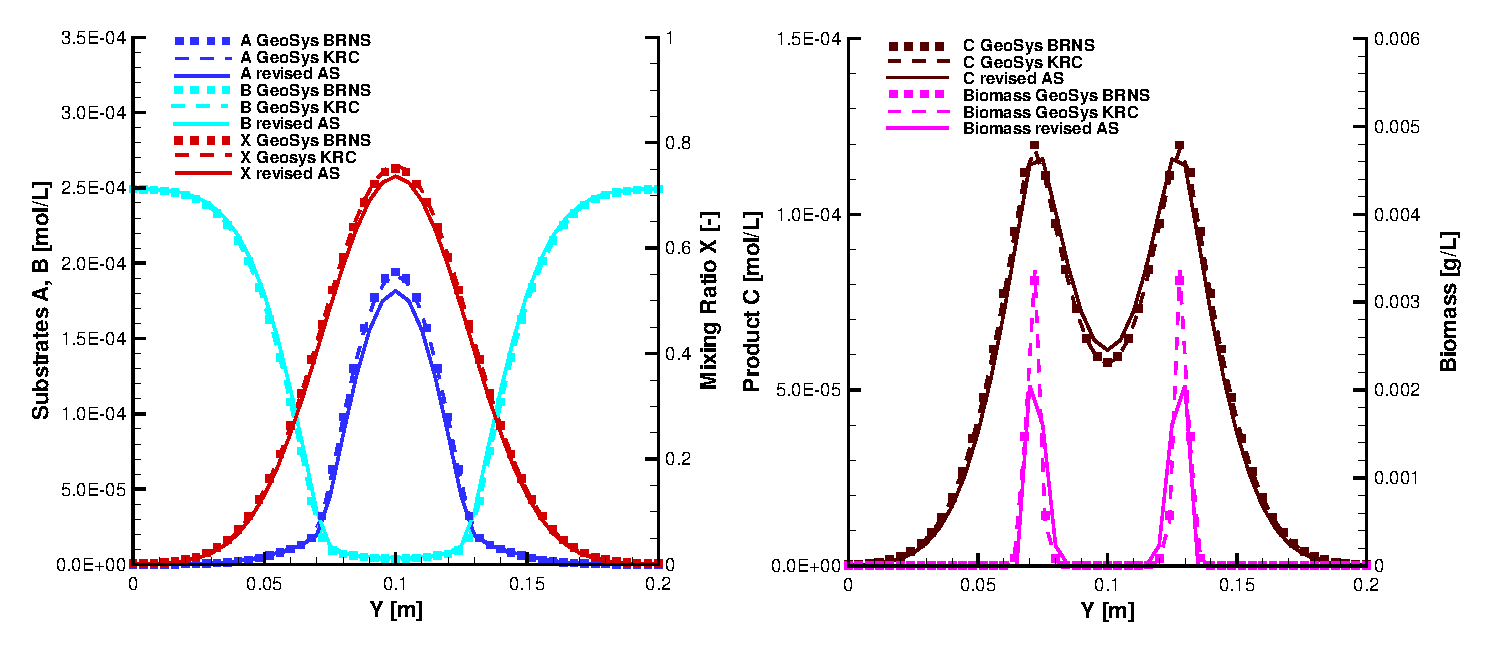
\includegraphics[scale=0.5]{PART_III/HC/monod_2d_brns_gs_as.eps}
%  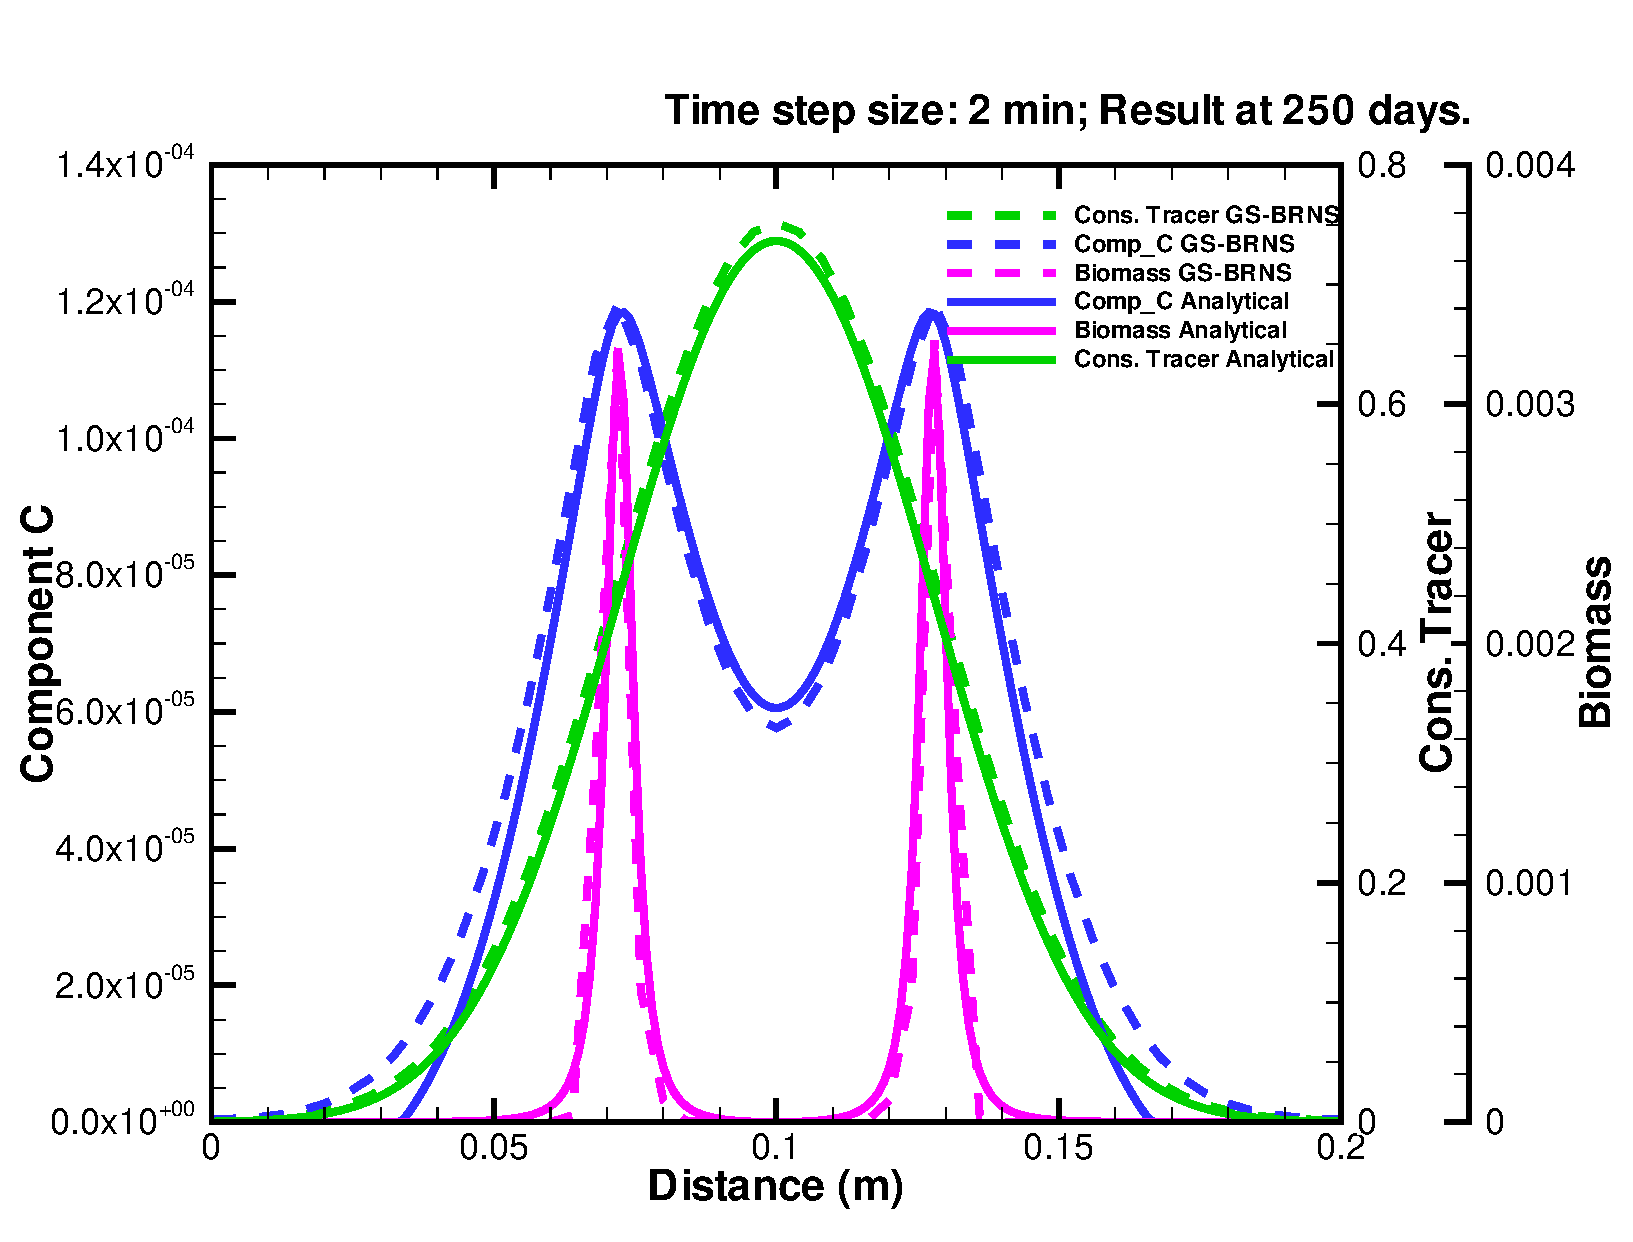
\includegraphics[scale=0.4]{C/figures/monod2d_tss2m_2.eps}
  \end{center}
  \caption{Simulation results for the transversal mixing model, using the
  kinetic approach and the finest temporal and spatial resolution. Analytical
  solution as solid lines, result of the numerical simulations with GeoSysBRNS as symbols and of GeoSysKRC as dashed lines.}
  \label{fig:monod2d_tss2m}
\end{figure}



